\documentclass[twoside]{book}

% Packages required by doxygen
\usepackage{fixltx2e}
\usepackage{calc}
\usepackage{doxygen}
\usepackage[export]{adjustbox} % also loads graphicx
\usepackage{graphicx}
\usepackage[utf8]{inputenc}
\usepackage{makeidx}
\usepackage{multicol}
\usepackage{multirow}
\PassOptionsToPackage{warn}{textcomp}
\usepackage{textcomp}
\usepackage[nointegrals]{wasysym}
\usepackage[table]{xcolor}

% Font selection
\usepackage[T1]{fontenc}
\usepackage[scaled=.90]{helvet}
\usepackage{courier}
\usepackage{amssymb}
\usepackage{sectsty}
\renewcommand{\familydefault}{\sfdefault}
\allsectionsfont{%
  \fontseries{bc}\selectfont%
  \color{darkgray}%
}
\renewcommand{\DoxyLabelFont}{%
  \fontseries{bc}\selectfont%
  \color{darkgray}%
}
\newcommand{\+}{\discretionary{\mbox{\scriptsize$\hookleftarrow$}}{}{}}

% Page & text layout
\usepackage{geometry}
\geometry{%
  a4paper,%
  top=2.5cm,%
  bottom=2.5cm,%
  left=2.5cm,%
  right=2.5cm%
}
\tolerance=750
\hfuzz=15pt
\hbadness=750
\setlength{\emergencystretch}{15pt}
\setlength{\parindent}{0cm}
\setlength{\parskip}{0.2cm}
\makeatletter
\renewcommand{\paragraph}{%
  \@startsection{paragraph}{4}{0ex}{-1.0ex}{1.0ex}{%
    \normalfont\normalsize\bfseries\SS@parafont%
  }%
}
\renewcommand{\subparagraph}{%
  \@startsection{subparagraph}{5}{0ex}{-1.0ex}{1.0ex}{%
    \normalfont\normalsize\bfseries\SS@subparafont%
  }%
}
\makeatother

% Headers & footers
\usepackage{fancyhdr}
\pagestyle{fancyplain}
\fancyhead[LE]{\fancyplain{}{\bfseries\thepage}}
\fancyhead[CE]{\fancyplain{}{}}
\fancyhead[RE]{\fancyplain{}{\bfseries\leftmark}}
\fancyhead[LO]{\fancyplain{}{\bfseries\rightmark}}
\fancyhead[CO]{\fancyplain{}{}}
\fancyhead[RO]{\fancyplain{}{\bfseries\thepage}}
\fancyfoot[LE]{\fancyplain{}{}}
\fancyfoot[CE]{\fancyplain{}{}}
\fancyfoot[RE]{\fancyplain{}{\bfseries\scriptsize Generated on Fri Jan 12 2018 00\+:27\+:21 for Roll-\/a-\/ball by Doxygen }}
\fancyfoot[LO]{\fancyplain{}{\bfseries\scriptsize Generated on Fri Jan 12 2018 00\+:27\+:21 for Roll-\/a-\/ball by Doxygen }}
\fancyfoot[CO]{\fancyplain{}{}}
\fancyfoot[RO]{\fancyplain{}{}}
\renewcommand{\footrulewidth}{0.4pt}
\renewcommand{\chaptermark}[1]{%
  \markboth{#1}{}%
}
\renewcommand{\sectionmark}[1]{%
  \markright{\thesection\ #1}%
}

% Indices & bibliography
\usepackage{natbib}
\usepackage[titles]{tocloft}
\setcounter{tocdepth}{3}
\setcounter{secnumdepth}{5}
\makeindex

% Hyperlinks (required, but should be loaded last)
\usepackage{ifpdf}
\ifpdf
  \usepackage[pdftex,pagebackref=true]{hyperref}
\else
  \usepackage[ps2pdf,pagebackref=true]{hyperref}
\fi
\hypersetup{%
  colorlinks=true,%
  linkcolor=blue,%
  citecolor=blue,%
  unicode%
}

% Custom commands
\newcommand{\clearemptydoublepage}{%
  \newpage{\pagestyle{empty}\cleardoublepage}%
}


%===== C O N T E N T S =====

\begin{document}

% Titlepage & ToC
\hypersetup{pageanchor=false,
             bookmarks=true,
             bookmarksnumbered=true,
             pdfencoding=unicode
            }
\pagenumbering{roman}
\begin{titlepage}
\vspace*{7cm}
\begin{center}%
{\Large Roll-\/a-\/ball }\\
\vspace*{1cm}
{\large Generated by Doxygen 1.8.9}\\
\vspace*{0.5cm}
{\small Fri Jan 12 2018 00:27:21}\\
\end{center}
\end{titlepage}
\clearemptydoublepage
\tableofcontents
\clearemptydoublepage
\pagenumbering{arabic}
\hypersetup{pageanchor=true}

%--- Begin generated contents ---
\chapter{Hierarchical Index}
\section{Class Hierarchy}
This inheritance list is sorted roughly, but not completely, alphabetically\+:\begin{DoxyCompactList}
\item Mono\+Behaviour\begin{DoxyCompactList}
\item \contentsline{section}{Camera\+Controller}{\pageref{class_camera_controller}}{}
\item \contentsline{section}{Player\+Controller}{\pageref{class_player_controller}}{}
\item \contentsline{section}{Rotator}{\pageref{class_rotator}}{}
\end{DoxyCompactList}
\end{DoxyCompactList}

\chapter{Class Index}
\section{Class List}
Here are the classes, structs, unions and interfaces with brief descriptions\+:\begin{DoxyCompactList}
\item\contentsline{section}{\hyperlink{class_camera_controller}{Camera\+Controller} \\*Controlador del Game\+Object Main Camera }{\pageref{class_camera_controller}}{}
\item\contentsline{section}{\hyperlink{class_player_controller}{Player\+Controller} \\*Controlador del Game\+Object Player. }{\pageref{class_player_controller}}{}
\item\contentsline{section}{\hyperlink{class_rotator}{Rotator} \\*Script que hace la animacion de girar a los Pick\+Ups. }{\pageref{class_rotator}}{}
\end{DoxyCompactList}

\chapter{File Index}
\section{File List}
Here is a list of all files with brief descriptions\+:\begin{DoxyCompactList}
\item\contentsline{section}{Scripts/\hyperlink{_camera_controller_8cs}{Camera\+Controller.\+cs} }{\pageref{_camera_controller_8cs}}{}
\item\contentsline{section}{Scripts/\hyperlink{_player_controller_8cs}{Player\+Controller.\+cs} }{\pageref{_player_controller_8cs}}{}
\item\contentsline{section}{Scripts/\hyperlink{_rotator_8cs}{Rotator.\+cs} }{\pageref{_rotator_8cs}}{}
\end{DoxyCompactList}

\chapter{Class Documentation}
\hypertarget{class_camera_controller}{}\section{Camera\+Controller Class Reference}
\label{class_camera_controller}\index{Camera\+Controller@{Camera\+Controller}}


Controlador del Game\+Object Main Camera  


Inheritance diagram for Camera\+Controller\+:\begin{figure}[H]
\begin{center}
\leavevmode
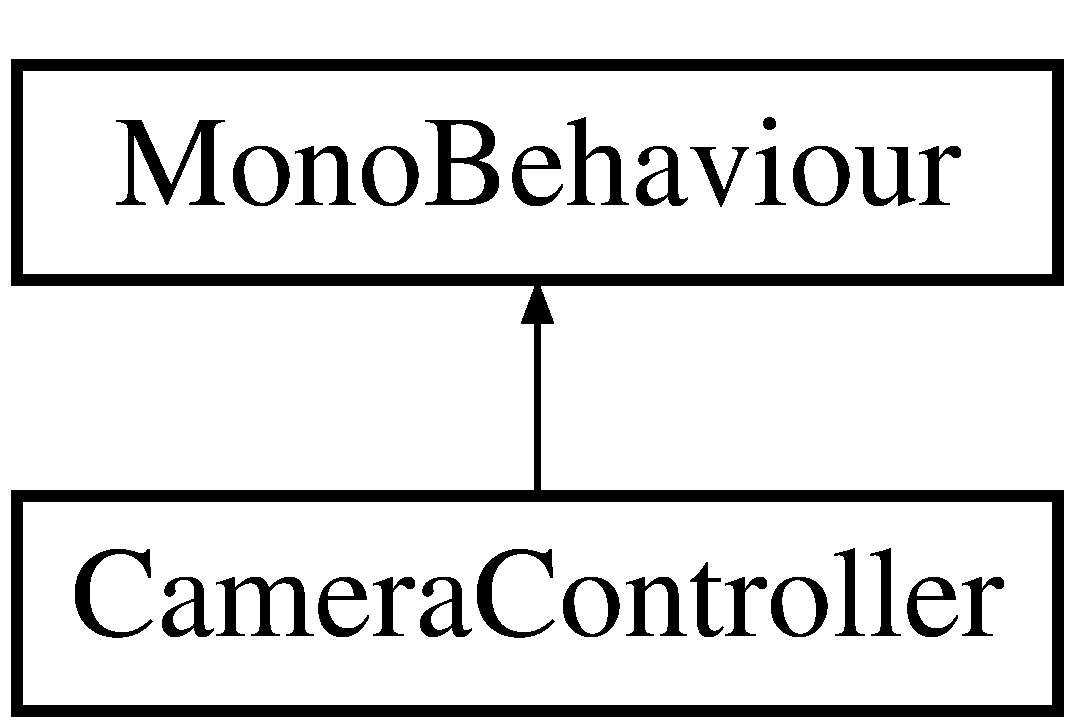
\includegraphics[height=2.000000cm]{class_camera_controller}
\end{center}
\end{figure}
\subsection*{Public Attributes}
\begin{DoxyCompactItemize}
\item 
Game\+Object \hyperlink{class_camera_controller_aae794ec2d17947f671ce0eaef9aac8b7}{player}
\begin{DoxyCompactList}\small\item\em Game\+Object Player al que vamos a tomar como referencia. \end{DoxyCompactList}\end{DoxyCompactItemize}
\subsection*{Private Member Functions}
\begin{DoxyCompactItemize}
\item 
void \hyperlink{class_camera_controller_ad4a238c6f7db3ee003302a245d860860}{Start} ()
\begin{DoxyCompactList}\small\item\em Metodo que es llamado nada mas iniciar el juego. \end{DoxyCompactList}\item 
void \hyperlink{class_camera_controller_afcd241727886518c21b9609193e32d18}{Late\+Update} ()
\begin{DoxyCompactList}\small\item\em Metodo llamado despues de actualizar los datos en cada frame. \end{DoxyCompactList}\end{DoxyCompactItemize}
\subsection*{Private Attributes}
\begin{DoxyCompactItemize}
\item 
Vector3 \hyperlink{class_camera_controller_aff80d2275dae360196361c39078bfda4}{offset}
\begin{DoxyCompactList}\small\item\em Desfase de la posicion del Game\+Object a la de Player. \end{DoxyCompactList}\end{DoxyCompactItemize}


\subsection{Detailed Description}
Controlador del Game\+Object Main Camera 



\subsection{Member Function Documentation}
\hypertarget{class_camera_controller_afcd241727886518c21b9609193e32d18}{}\index{Camera\+Controller@{Camera\+Controller}!Late\+Update@{Late\+Update}}
\index{Late\+Update@{Late\+Update}!Camera\+Controller@{Camera\+Controller}}
\subsubsection[{Late\+Update}]{\setlength{\rightskip}{0pt plus 5cm}void Camera\+Controller.\+Late\+Update (
\begin{DoxyParamCaption}
{}
\end{DoxyParamCaption}
)\hspace{0.3cm}{\ttfamily [inline]}, {\ttfamily [private]}}\label{class_camera_controller_afcd241727886518c21b9609193e32d18}


Metodo llamado despues de actualizar los datos en cada frame. 

El frame ha refrescado la posicion del jugador. Ahora con esta nueva posicion vamos a situar la camara en su posicion equivalente segun el desfase calculado. \hypertarget{class_camera_controller_ad4a238c6f7db3ee003302a245d860860}{}\index{Camera\+Controller@{Camera\+Controller}!Start@{Start}}
\index{Start@{Start}!Camera\+Controller@{Camera\+Controller}}
\subsubsection[{Start}]{\setlength{\rightskip}{0pt plus 5cm}void Camera\+Controller.\+Start (
\begin{DoxyParamCaption}
{}
\end{DoxyParamCaption}
)\hspace{0.3cm}{\ttfamily [inline]}, {\ttfamily [private]}}\label{class_camera_controller_ad4a238c6f7db3ee003302a245d860860}


Metodo que es llamado nada mas iniciar el juego. 

Restamos a la posicion de la camara la del jugador. 

\subsection{Member Data Documentation}
\hypertarget{class_camera_controller_aff80d2275dae360196361c39078bfda4}{}\index{Camera\+Controller@{Camera\+Controller}!offset@{offset}}
\index{offset@{offset}!Camera\+Controller@{Camera\+Controller}}
\subsubsection[{offset}]{\setlength{\rightskip}{0pt plus 5cm}Vector3 Camera\+Controller.\+offset\hspace{0.3cm}{\ttfamily [private]}}\label{class_camera_controller_aff80d2275dae360196361c39078bfda4}


Desfase de la posicion del Game\+Object a la de Player. 

\hypertarget{class_camera_controller_aae794ec2d17947f671ce0eaef9aac8b7}{}\index{Camera\+Controller@{Camera\+Controller}!player@{player}}
\index{player@{player}!Camera\+Controller@{Camera\+Controller}}
\subsubsection[{player}]{\setlength{\rightskip}{0pt plus 5cm}Game\+Object Camera\+Controller.\+player}\label{class_camera_controller_aae794ec2d17947f671ce0eaef9aac8b7}


Game\+Object Player al que vamos a tomar como referencia. 



The documentation for this class was generated from the following file\+:\begin{DoxyCompactItemize}
\item 
Scripts/\hyperlink{_camera_controller_8cs}{Camera\+Controller.\+cs}\end{DoxyCompactItemize}

\hypertarget{class_player_controller}{}\section{Player\+Controller Class Reference}
\label{class_player_controller}\index{Player\+Controller@{Player\+Controller}}


Controlador del Game\+Object Player.  


Inheritance diagram for Player\+Controller\+:\begin{figure}[H]
\begin{center}
\leavevmode
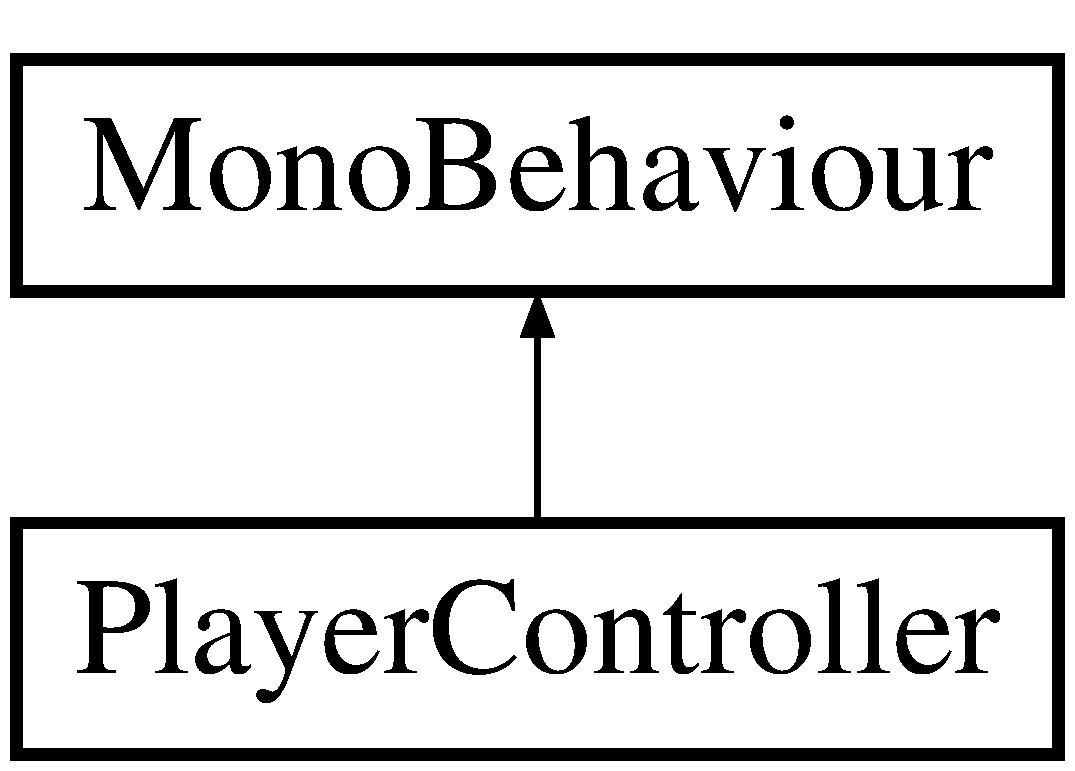
\includegraphics[height=2.000000cm]{class_player_controller}
\end{center}
\end{figure}
\subsection*{Public Attributes}
\begin{DoxyCompactItemize}
\item 
float \hyperlink{class_player_controller_a0928605583f0563cd84fe43119d336ec}{speed}
\begin{DoxyCompactList}\small\item\em Multiplicador de velocidad de la esfera. \end{DoxyCompactList}\item 
Text \hyperlink{class_player_controller_a61795bee5f0ca4705f688419919e3086}{count\+Text}
\begin{DoxyCompactList}\small\item\em Game\+Object de texto que indica la puntuación. \end{DoxyCompactList}\item 
Text \hyperlink{class_player_controller_a366f431ae274e7b19365f7b15b1709b8}{win\+Text}
\begin{DoxyCompactList}\small\item\em Game\+Object de texto que felicita al jugador. \end{DoxyCompactList}\end{DoxyCompactItemize}
\subsection*{Private Member Functions}
\begin{DoxyCompactItemize}
\item 
void \hyperlink{class_player_controller_ae1117d9c4da3193181cddad2c814e467}{Start} ()
\begin{DoxyCompactList}\small\item\em Metodo que es llamado nada mas inicar el juego. \end{DoxyCompactList}\item 
void \hyperlink{class_player_controller_ae5bdb1b48571f67c3f722a58b6f404d4}{Fixed\+Update} ()
\begin{DoxyCompactList}\small\item\em Metodo Update() especifico para el Rigidbody. \end{DoxyCompactList}\item 
void \hyperlink{class_player_controller_a2a0510e318c75ef04e45b4ece3bd31cd}{On\+Trigger\+Enter} (Collider other)
\begin{DoxyCompactList}\small\item\em Metodo que es llamado cada vez que el jugador interactua (colisiona con la hitbox) de otro Game\+Object que tenga algun componente de tipo Collider. \end{DoxyCompactList}\item 
void \hyperlink{class_player_controller_ad55b05bf5e6a5ae39a2a01700f1772ce}{Set\+Count\+Text} ()
\begin{DoxyCompactList}\small\item\em Metodo que actualiza la puntuacion que mostramos en pantalla con la puntuacion actual. \end{DoxyCompactList}\end{DoxyCompactItemize}
\subsection*{Private Attributes}
\begin{DoxyCompactItemize}
\item 
Rigidbody \hyperlink{class_player_controller_a93b9fa76e5456725594e87dd40f93611}{rb}
\begin{DoxyCompactList}\small\item\em Componente del Game\+Object para manejas las fisicas. \end{DoxyCompactList}\item 
int \hyperlink{class_player_controller_ac44590ddcba0af5af97eb025a56f9ae5}{count}
\begin{DoxyCompactList}\small\item\em La puntuacion actual. \end{DoxyCompactList}\end{DoxyCompactItemize}


\subsection{Detailed Description}
Controlador del Game\+Object Player. 



\subsection{Member Function Documentation}
\hypertarget{class_player_controller_ae5bdb1b48571f67c3f722a58b6f404d4}{}\index{Player\+Controller@{Player\+Controller}!Fixed\+Update@{Fixed\+Update}}
\index{Fixed\+Update@{Fixed\+Update}!Player\+Controller@{Player\+Controller}}
\subsubsection[{Fixed\+Update}]{\setlength{\rightskip}{0pt plus 5cm}void Player\+Controller.\+Fixed\+Update (
\begin{DoxyParamCaption}
{}
\end{DoxyParamCaption}
)\hspace{0.3cm}{\ttfamily [inline]}, {\ttfamily [private]}}\label{class_player_controller_ae5bdb1b48571f67c3f722a58b6f404d4}


Metodo Update() especifico para el Rigidbody. 

Asignamos el valor del control Izquierda/\+Derecha.

Asignamos el valor del control Arriba/\+Abajo.

Aplicamos una fuerza a la direccion de los controles segun el valor de speed. \hypertarget{class_player_controller_a2a0510e318c75ef04e45b4ece3bd31cd}{}\index{Player\+Controller@{Player\+Controller}!On\+Trigger\+Enter@{On\+Trigger\+Enter}}
\index{On\+Trigger\+Enter@{On\+Trigger\+Enter}!Player\+Controller@{Player\+Controller}}
\subsubsection[{On\+Trigger\+Enter}]{\setlength{\rightskip}{0pt plus 5cm}void Player\+Controller.\+On\+Trigger\+Enter (
\begin{DoxyParamCaption}
\item[{Collider}]{other}
\end{DoxyParamCaption}
)\hspace{0.3cm}{\ttfamily [inline]}, {\ttfamily [private]}}\label{class_player_controller_a2a0510e318c75ef04e45b4ece3bd31cd}


Metodo que es llamado cada vez que el jugador interactua (colisiona con la hitbox) de otro Game\+Object que tenga algun componente de tipo Collider. 


\begin{DoxyParams}{Parameters}
{\em other} & El componente Collider del Gameobject con el que colisiona.\\
\hline
\end{DoxyParams}
Comprobamos que el Game\+Object con el que colisiona tenga la tag \char`\"{}\+Pick\+Up\char`\"{}.

Deshabilitamos el Game\+O\+Bject.

Ganamos un punto.

Actualizamos la puntuacion en pantalla. \hypertarget{class_player_controller_ad55b05bf5e6a5ae39a2a01700f1772ce}{}\index{Player\+Controller@{Player\+Controller}!Set\+Count\+Text@{Set\+Count\+Text}}
\index{Set\+Count\+Text@{Set\+Count\+Text}!Player\+Controller@{Player\+Controller}}
\subsubsection[{Set\+Count\+Text}]{\setlength{\rightskip}{0pt plus 5cm}void Player\+Controller.\+Set\+Count\+Text (
\begin{DoxyParamCaption}
{}
\end{DoxyParamCaption}
)\hspace{0.3cm}{\ttfamily [inline]}, {\ttfamily [private]}}\label{class_player_controller_ad55b05bf5e6a5ae39a2a01700f1772ce}


Metodo que actualiza la puntuacion que mostramos en pantalla con la puntuacion actual. 

Actualizamos el Game\+Object count\+Text con la puntuacion actual.

Y si la puntuacion actual es de 6 (Puntuacion maxima).

Felicitamos al jugador con un Game Over. \hypertarget{class_player_controller_ae1117d9c4da3193181cddad2c814e467}{}\index{Player\+Controller@{Player\+Controller}!Start@{Start}}
\index{Start@{Start}!Player\+Controller@{Player\+Controller}}
\subsubsection[{Start}]{\setlength{\rightskip}{0pt plus 5cm}void Player\+Controller.\+Start (
\begin{DoxyParamCaption}
{}
\end{DoxyParamCaption}
)\hspace{0.3cm}{\ttfamily [inline]}, {\ttfamily [private]}}\label{class_player_controller_ae1117d9c4da3193181cddad2c814e467}


Metodo que es llamado nada mas inicar el juego. 

Asignamos el componente Rigidbody del Game\+Object.

Ponemos el contador a cero.

Ponemos la puntuacion en pantalla. 

\subsection{Member Data Documentation}
\hypertarget{class_player_controller_ac44590ddcba0af5af97eb025a56f9ae5}{}\index{Player\+Controller@{Player\+Controller}!count@{count}}
\index{count@{count}!Player\+Controller@{Player\+Controller}}
\subsubsection[{count}]{\setlength{\rightskip}{0pt plus 5cm}int Player\+Controller.\+count\hspace{0.3cm}{\ttfamily [private]}}\label{class_player_controller_ac44590ddcba0af5af97eb025a56f9ae5}


La puntuacion actual. 

\hypertarget{class_player_controller_a61795bee5f0ca4705f688419919e3086}{}\index{Player\+Controller@{Player\+Controller}!count\+Text@{count\+Text}}
\index{count\+Text@{count\+Text}!Player\+Controller@{Player\+Controller}}
\subsubsection[{count\+Text}]{\setlength{\rightskip}{0pt plus 5cm}Text Player\+Controller.\+count\+Text}\label{class_player_controller_a61795bee5f0ca4705f688419919e3086}


Game\+Object de texto que indica la puntuación. 

\hypertarget{class_player_controller_a93b9fa76e5456725594e87dd40f93611}{}\index{Player\+Controller@{Player\+Controller}!rb@{rb}}
\index{rb@{rb}!Player\+Controller@{Player\+Controller}}
\subsubsection[{rb}]{\setlength{\rightskip}{0pt plus 5cm}Rigidbody Player\+Controller.\+rb\hspace{0.3cm}{\ttfamily [private]}}\label{class_player_controller_a93b9fa76e5456725594e87dd40f93611}


Componente del Game\+Object para manejas las fisicas. 

\hypertarget{class_player_controller_a0928605583f0563cd84fe43119d336ec}{}\index{Player\+Controller@{Player\+Controller}!speed@{speed}}
\index{speed@{speed}!Player\+Controller@{Player\+Controller}}
\subsubsection[{speed}]{\setlength{\rightskip}{0pt plus 5cm}float Player\+Controller.\+speed}\label{class_player_controller_a0928605583f0563cd84fe43119d336ec}


Multiplicador de velocidad de la esfera. 

\hypertarget{class_player_controller_a366f431ae274e7b19365f7b15b1709b8}{}\index{Player\+Controller@{Player\+Controller}!win\+Text@{win\+Text}}
\index{win\+Text@{win\+Text}!Player\+Controller@{Player\+Controller}}
\subsubsection[{win\+Text}]{\setlength{\rightskip}{0pt plus 5cm}Text Player\+Controller.\+win\+Text}\label{class_player_controller_a366f431ae274e7b19365f7b15b1709b8}


Game\+Object de texto que felicita al jugador. 



The documentation for this class was generated from the following file\+:\begin{DoxyCompactItemize}
\item 
Scripts/\hyperlink{_player_controller_8cs}{Player\+Controller.\+cs}\end{DoxyCompactItemize}

\hypertarget{class_rotator}{}\section{Rotator Class Reference}
\label{class_rotator}\index{Rotator@{Rotator}}


Script que hace la animacion de girar a los Pick\+Ups.  


Inheritance diagram for Rotator\+:\begin{figure}[H]
\begin{center}
\leavevmode
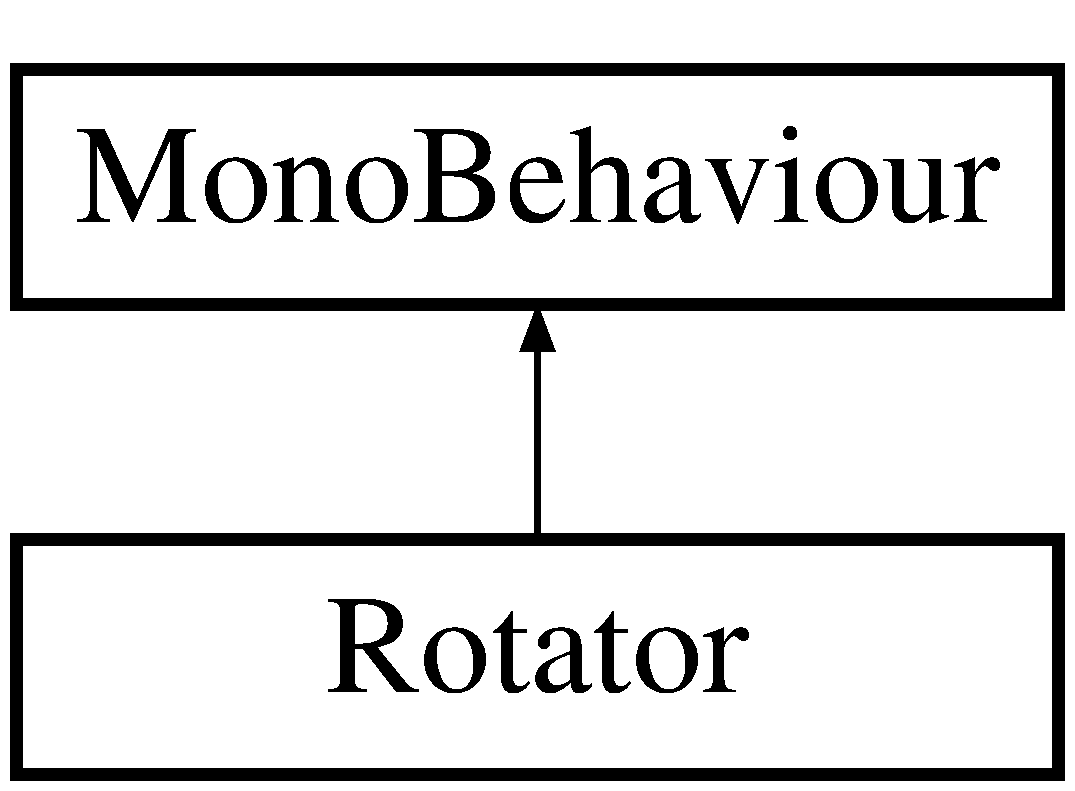
\includegraphics[height=2.000000cm]{class_rotator}
\end{center}
\end{figure}
\subsection*{Private Member Functions}
\begin{DoxyCompactItemize}
\item 
void \hyperlink{class_rotator_a5b573a6122b39499ebd67d6db7c905e9}{Update} ()
\begin{DoxyCompactList}\small\item\em Metodo llamado una vez por cada frame. \end{DoxyCompactList}\end{DoxyCompactItemize}


\subsection{Detailed Description}
Script que hace la animacion de girar a los Pick\+Ups. 



\subsection{Member Function Documentation}
\hypertarget{class_rotator_a5b573a6122b39499ebd67d6db7c905e9}{}\index{Rotator@{Rotator}!Update@{Update}}
\index{Update@{Update}!Rotator@{Rotator}}
\subsubsection[{Update}]{\setlength{\rightskip}{0pt plus 5cm}void Rotator.\+Update (
\begin{DoxyParamCaption}
{}
\end{DoxyParamCaption}
)\hspace{0.3cm}{\ttfamily [inline]}, {\ttfamily [private]}}\label{class_rotator_a5b573a6122b39499ebd67d6db7c905e9}


Metodo llamado una vez por cada frame. 

Giramos al Game\+Object 12 grados hacia la izquierda, 30 grados hacia arriba y 45 grados hacia atras, multiplicado por el tiempo en segundos que ha pasado desde el anterior frame. 

The documentation for this class was generated from the following file\+:\begin{DoxyCompactItemize}
\item 
Scripts/\hyperlink{_rotator_8cs}{Rotator.\+cs}\end{DoxyCompactItemize}

\chapter{File Documentation}
\hypertarget{_camera_controller_8cs}{}\section{Scripts/\+Camera\+Controller.cs File Reference}
\label{_camera_controller_8cs}\index{Scripts/\+Camera\+Controller.\+cs@{Scripts/\+Camera\+Controller.\+cs}}
\subsection*{Classes}
\begin{DoxyCompactItemize}
\item 
class \hyperlink{class_camera_controller}{Camera\+Controller}
\begin{DoxyCompactList}\small\item\em Controlador del Game\+Object Main Camera \end{DoxyCompactList}\end{DoxyCompactItemize}

\hypertarget{_player_controller_8cs}{}\section{Scripts/\+Player\+Controller.cs File Reference}
\label{_player_controller_8cs}\index{Scripts/\+Player\+Controller.\+cs@{Scripts/\+Player\+Controller.\+cs}}
\subsection*{Classes}
\begin{DoxyCompactItemize}
\item 
class \hyperlink{class_player_controller}{Player\+Controller}
\begin{DoxyCompactList}\small\item\em Controlador del Game\+Object Player. \end{DoxyCompactList}\end{DoxyCompactItemize}

\hypertarget{_rotator_8cs}{}\section{Scripts/\+Rotator.cs File Reference}
\label{_rotator_8cs}\index{Scripts/\+Rotator.\+cs@{Scripts/\+Rotator.\+cs}}
\subsection*{Classes}
\begin{DoxyCompactItemize}
\item 
class \hyperlink{class_rotator}{Rotator}
\begin{DoxyCompactList}\small\item\em Script que hace la animacion de girar a los Pick\+Ups. \end{DoxyCompactList}\end{DoxyCompactItemize}

%--- End generated contents ---

% Index
\backmatter
\newpage
\phantomsection
\clearemptydoublepage
\addcontentsline{toc}{chapter}{Index}
\printindex

\end{document}
